El Trabajo de Fin de Máster (TFM) consta de 12 créditos ECTS, lo que equivale a
unas 300 horas de dedicación total, considerando que 1 ECTS representa entre 25
y 27 horas de trabajo. Este tiempo abarca todas las actividades necesarias para
la realización del TFM, incluyendo investigación, redacción, desarrollo
técnico, reunión con el supervisor, preparación de la defensa y demás tareas
asociadas al proyecto.

\subsection{Planificación Temporal}

La planificación temporal del proyecto se organiza en varias fases o etapas.
Cada una de ellas es necesaria para el cumplimiento de los objetivos
establecidos.

\begin{itemize}

	\item \textbf{Fase 1: Definición del tema y objetivos}.
	      Semanas 1-2, estimadas 30 horas.

	\item \textbf{Fase 2: Revisión de literatura y estado del arte}.
	      Semanas 3-4, estimadas 40 horas.

	\item \textbf{Fase 3: Desarrollo del proyecto}.
	      Semanas 5-11, estimadas 150 horas.

	\item \textbf{Fase 4: Redacción del informe final}.
	      Semanas 12-15, estimadas 50 horas.

	\item \textbf{Fase 5: Revisión y preparación de la defensa}.
	      Semanas 16-17, estimadas 30 horas.

\end{itemize}

\subsection{Coste}

El trabajo de 300 horas totales se valora sobre la base de un sueldo medio de
ingeniero junior en energías renovables en Madrid, que ronda los 25000-31000
euros brutos anuales
\footnote{\url{https://www.adecco.es/guia-salarial/guia-salarial-2024-energeticas}}
(figura \ref{fig:engineer_wage}). Tomando una media de 28000 euros, y
considerando que se trabajan unas 40 horas a la semana, por 52 semanas que
tiene el año, calculamos el coste por hora.

\begin{figure}[h] \centering
	\centering
	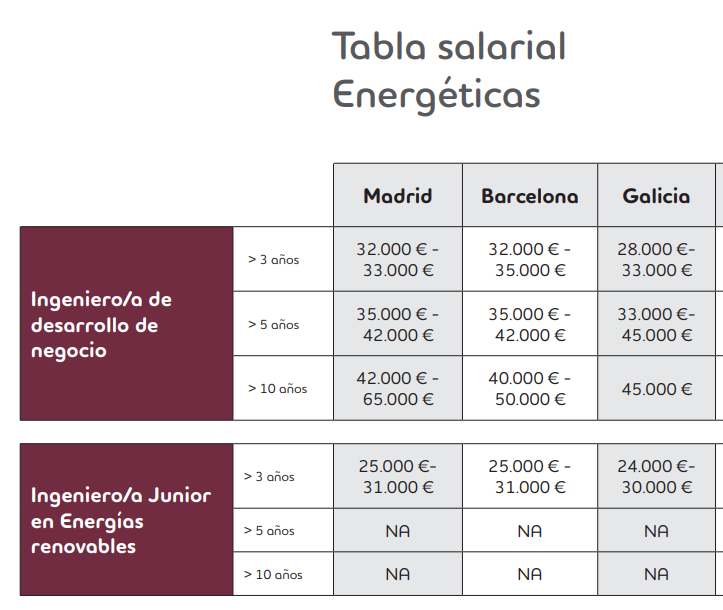
\includegraphics[width=0.7\textwidth]{./capitulos/planificacion_presupuesto/images/engineer_wage.png}
	\caption{Sueldos para ingeniero junior en energías renovables, según la guía salarial de adecco para 2024.}
	\label{fig:engineer_wage}
\end{figure}

\begin{equation}
	28000 \left[\frac{\text{\euro}}{\text{año}} \right] \cdot \frac{1}{40} \left[\frac{\text{semana}}{\text{hora}}\right] \cdot \frac{1}{52} \left[\frac{\text{año}}{\text{semana}}\right] = 13.46 \left[\frac{\text{\euro}}{\text{hora}}\right]
\end{equation}

Y multiplicando el coste por hora por las horas totales del proyecto, tenemos
el coste total:

\begin{equation}
	300 [\text{hora}] \cdot 13.46 \left[\frac{\text{\euro}}{\text{hora}}\right] = 4038 [\text{\euro}]
\end{equation}

Este valor monetario da una idea del esfuerzo y la dedicación necesarios para
un proyecto de fin de máster.
